\documentclass{article}
\title{The regressx1 data}
\usepackage{Statweave}
\begin{document}
\maketitle
The data:
\begin{verbatim}
subjno timedrs phyheal menheal stress 
1 1 5 8 265 
2 3 4 6 415 
3 0 3 4 92 
4 13 2 2 241 
5 15 3 6 86 
6 3 5 5 247 
7 2 5 6 13 
8 0 4 5 12 
9 7 5 4 269 
10 4 3 9 391 
11 15 6 3 237 
12 0 3 5 13 
13 2 3 10 84 
14 13 6 9 144 
15 2 3 2 135 
16 2 3 4 291 
21 1 3 1 98 
22 2 7 8 233 
23 5 4 6 147 
24 5 7 13 308 
25 3 4 12 122 
26 4 2 3 307 
27 2 3 4 248 
28 0 5 14 122 
29 13 7 10 384 
30 7 8 11 433 
31 2 6 9 260 
32 12 9 12 313 
33 2 3 8 400 
34 5 7 9 328 
35 4 8 4 266 
36 6 8 14 422 
37 2 6 16 101 
38 3 4 11 168 
39 14 9 12 402 
40 7 8 10 302 
45 0 6 0 83 
46 1 2 7 244 
47 3 3 6 171 
48 60 7 6 271 
49 5 2 0 53 
50 3 5 4 59 
51 0 7 6 85 
52 3 5 10 64 
53 2 2 0 338 
54 1 2 4 134 
55 1 2 1 70 
56 13 8 12 320 
57 2 2 1 91 
65 5 8 6 270 
66 12 7 12 136 
67 12 10 18 142 
68 1 2 4 259 
69 20 3 6 174 
70 0 2 3 13 
71 5 5 3 390 
72 0 3 3 242 
73 8 6 3 103 
74 9 5 5 338 
75 10 9 8 436 
76 1 4 3 120 
77 5 4 7 361 
78 5 4 4 293 
79 23 12 4 237 
80 7 8 15 244 
81 1 2 4 181 
82 39 4 7 265 
83 2 2 1 38 
84 7 5 5 157 
85 9 4 10 197 
86 0 6 11 159 
87 4 5 5 75 
88 16 10 5 207 
89 0 4 4 83 
90 16 3 11 222 
91 33 4 6 200 
95 4 6 11 251 
97 2 3 6 218 
98 38 12 11 237 
99 8 4 7 139 
101 2 8 12 464 
102 2 3 5 128 
103 0 2 1 0 
104 15 8 8 334 
105 0 3 0 55 
106 1 2 2 169 
107 5 5 9 77 
108 7 4 3 112 
109 10 6 3 164 
110 22 7 8 172 
111 10 4 7 271 
112 0 3 2 69 
113 11 3 2 106 
114 9 3 1 214 
115 0 2 1 10 
116 34 10 15 321 
117 3 3 4 172 
118 1 2 8 320 
119 0 4 0 26 
120 10 8 11 194 
121 4 2 1 122 
122 27 6 13 565 
123 7 8 18 433 
124 1 3 2 314 
125 7 6 4 129 
126 3 5 10 209 
127 2 4 10 417 
128 11 6 13 427 
129 9 5 5 179 
130 11 8 15 174 
131 11 5 12 361 
132 8 6 5 107 
133 2 7 18 338 
134 4 4 8 197 
135 4 5 1 44 
136 6 5 6 345 
137 30 11 9 238 
138 7 6 11 225 
139 15 9 8 531 
140 6 11 12 206 
141 7 7 6 68 
142 2 5 3 12 
143 1 2 2 155 
144 5 5 8 220 
145 1 3 16 377 
146 11 7 1 241 
148 16 8 7 165 
149 2 2 1 356 
150 14 6 5 81 
151 8 5 9 81 
152 17 8 15 169 
153 1 2 6 168 
154 0 2 2 72 
155 1 2 0 105 
156 1 3 2 41 
157 10 7 16 334 
158 7 6 13 282 
159 2 3 0 93 
160 5 4 5 227 
166 6 4 12 310 
167 1 3 1 265 
183 16 9 12 272 
184 0 6 5 207 
185 17 11 17 534 
187 0 4 1 169 
190 10 3 8 577 
192 6 8 2 236 
202 20 7 5 62 
203 1 3 3 64 
204 25 4 6 160 
205 3 5 3 130 
206 6 3 0 270 
208 0 2 0 50 
210 8 5 10 149 
212 9 9 4 312 
213 19 7 10 303 
214 2 2 0 133 
225 2 3 7 278 
226 3 2 0 441 
227 7 4 5 253 
228 2 4 16 256 
229 8 6 5 127 
230 49 10 9 113 
231 2 3 7 221 
232 1 2 6 279 
233 5 6 7 189 
234 5 3 13 282 
235 60 6 11 529 
236 10 4 2 236 
237 27 3 8 392 
238 7 6 8 216 
239 8 5 8 13 
240 12 5 0 245 
241 2 3 1 194 
242 2 3 3 74 
243 4 4 2 306 
244 6 7 9 235 
245 27 12 12 304 
246 0 2 5 352 
247 9 10 8 98 
248 3 2 5 75 
249 0 4 4 128 
250 2 3 4 171 
251 3 3 4 82 
252 5 4 1 268 
253 5 6 9 100 
254 1 4 6 271 
255 7 6 4 112 
258 4 6 5 301 
259 3 5 4 174 
260 7 6 7 336 
261 1 2 6 63 
262 52 6 6 225 
263 6 6 6 421 
264 18 8 7 597 
265 14 5 2 13 
266 0 3 6 71 
267 8 8 17 88 
268 16 5 1 20 
269 2 4 3 94 
270 12 6 5 174 
271 3 6 1 214 
272 24 8 8 147 
273 0 3 2 80 
274 0 4 1 69 
276 57 11 4 268 
277 11 8 13 138 
278 1 4 6 196 
279 18 9 10 546 
280 1 2 1 112 
289 11 4 7 265 
290 0 4 2 254 
291 52 6 2 156 
292 12 7 8 257 
293 6 5 6 170 
294 0 2 7 160 
295 2 3 2 426 
299 2 5 12 159 
300 13 5 13 104 
301 2 3 0 59 
302 3 5 1 63 
303 2 5 3 185 
304 2 6 10 211 
305 1 8 11 358 
306 2 2 0 69 
307 3 5 1 488 
308 1 3 4 89 
309 5 4 6 330 
310 6 6 9 67 
311 1 4 3 76 
312 2 3 3 391 
313 3 4 1 202 
314 7 6 13 126 
315 7 6 5 82 
316 0 2 1 164 
317 7 5 13 81 
318 8 9 1 143 
319 9 7 4 204 
320 8 2 5 97 
321 1 3 7 152 
322 14 7 13 160 
323 2 4 4 79 
324 4 3 6 102 
325 8 3 11 520 
326 3 4 5 88 
327 10 5 9 162 
328 21 9 16 191 
329 6 6 7 380 
330 58 5 6 328 
335 12 9 7 215 
336 5 3 4 183 
337 2 3 4 444 
338 2 6 11 122 
339 4 7 10 197 
340 2 4 4 153 
341 5 6 9 178 
342 0 2 0 0 
343 3 2 5 177 
344 7 5 3 371 
345 1 6 10 308 
346 2 2 5 33 
347 1 3 7 278 
348 4 3 7 356 
349 4 5 4 191 
355 4 2 6 234 
357 2 3 6 101 
358 0 3 10 186 
359 13 5 3 275 
361 3 7 9 139 
362 1 3 7 37 
363 4 5 8 364 
365 1 3 0 25 
367 3 4 3 226 
369 1 4 6 180 
370 57 6 13 85 
372 1 2 4 49 
374 17 15 10 258 
378 11 8 5 99 
379 43 4 9 567 
380 6 7 1 13 
381 6 6 5 282 
382 1 3 1 171 
383 0 3 6 114 
384 10 11 7 266 
385 3 6 1 159 
386 37 4 14 263 
387 6 3 1 236 
392 11 6 2 129 
397 4 3 0 98 
398 75 9 12 244 
399 7 6 12 547 
400 3 6 15 347 
401 3 6 13 309 
402 3 5 9 264 
403 4 4 5 66 
404 5 5 7 330 
405 2 5 0 90 
406 4 6 3 462 
407 2 2 4 77 
413 11 7 15 432 
414 0 3 8 212 
417 2 7 6 228 
418 4 4 2 326 
420 6 8 10 594 
421 0 5 4 87 
424 2 4 5 440 
425 5 7 7 77 
434 2 5 8 63 
435 10 7 12 389 
436 29 9 14 333 
437 3 7 9 99 
438 0 3 7 241 
439 21 3 8 476 
440 0 3 6 41 
441 3 3 4 17 
442 1 3 6 122 
443 9 4 3 337 
444 3 4 10 188 
445 3 3 3 228 
446 5 11 7 263 
447 6 4 2 139 
448 4 5 4 208 
451 16 5 5 101 
452 3 5 2 278 
453 13 8 8 331 
454 3 3 5 151 
455 2 4 4 135 
456 2 4 1 0 
457 3 5 1 208 
458 7 3 2 181 
459 2 3 0 104 
460 2 3 1 76 
461 2 2 0 211 
462 2 3 3 39 
463 5 5 1 150 
464 3 4 3 210 
465 2 3 0 15 
466 4 6 4 131 
467 1 2 0 0 
469 3 3 0 205 
472 6 4 2 163 
473 4 5 2 201 
474 30 6 1 224 
476 0 2 0 69 
479 25 2 2 62 
480 0 5 1 62 
481 5 3 3 204 
482 3 4 5 162 
483 2 2 5 221 
484 2 2 2 221 
485 9 12 6 348 
486 2 3 0 341 
487 13 3 3 336 
488 1 3 6 343 
489 4 6 6 177 
490 4 3 8 274 
491 3 4 4 290 
492 7 10 2 174 
493 7 5 5 111 
494 14 3 2 246 
495 4 4 7 181 
496 15 6 10 336 
497 37 7 5 55 
498 2 4 8 178 
499 4 3 6 98 
500 6 5 12 85 
501 10 5 1 66 
502 56 8 2 316 
503 3 4 4 139 
504 0 2 2 28 
505 18 10 15 421 
506 3 4 5 237 
507 18 14 16 494 
508 7 4 8 66 
509 29 9 3 93 
510 0 2 7 90 
511 5 6 8 227 
512 4 5 6 273 
513 3 5 11 171 
514 6 6 8 76 
515 21 13 12 404 
516 1 2 5 12 
517 3 2 8 380 
518 3 3 3 101 
519 0 2 2 68 
520 13 7 12 282 
521 5 3 5 0 
522 5 4 5 277 
523 37 9 15 392 
524 2 4 1 49 
525 11 13 16 372 
526 13 6 12 482 
527 2 2 1 81 
528 4 5 5 76 
529 21 7 11 329 
530 2 4 6 12 
533 4 4 10 158 
534 3 4 5 15 
535 3 8 5 105 
536 12 5 7 266 
538 1 2 2 0 
539 4 3 2 396 
540 13 9 7 920 
547 2 3 4 153 
548 81 5 7 731 
549 12 4 3 364 
550 2 2 3 33 
551 16 6 8 386 
552 27 9 6 79 
553 2 6 10 320 
554 2 4 1 178 
555 8 6 5 108 
556 2 3 1 157 
557 4 4 6 12 
558 3 3 3 25 
559 19 6 6 104 
560 4 3 3 91 
567 1 2 4 291 
568 3 2 8 85 
569 15 7 4 25 
570 4 5 6 130 
571 4 3 3 147 
572 13 10 12 155 
573 6 3 4 108 
574 1 5 9 523 
575 3 7 8 53 
576 3 5 6 306 
577 0 5 6 171 
578 22 7 5 158 
579 4 3 3 25 
580 14 6 4 398 
581 6 6 13 252 
582 16 5 14 538 
583 6 5 7 124 
584 0 3 7 75 
585 8 5 15 237 
586 0 3 4 118 
587 4 5 7 302 
588 5 8 10 170 
589 2 2 1 171 
590 6 4 7 73 
591 11 4 10 176 
592 1 4 3 176 
593 23 8 11 643 
683 4 4 12 179 
685 4 6 2 0 
686 16 8 14 132 
687 6 4 3 159 
688 1 2 4 110 
689 2 3 6 75 
690 6 9 10 272 
691 6 6 5 152 
706 3 4 12 119 
707 1 2 0 52 
708 15 6 12 252 
709 3 4 9 234 
710 7 7 4 214 
711 9 4 1 183 
717 18 6 10 166 
724 14 8 9 331 
754 3 3 6 73 
755 4 4 0 66 
756 15 9 6 142 
757 4 6 4 87 
758 3 5 2 149 
\end{verbatim}
The SAS code and output:
\begin{Winput}
data regr;
  infile "regressx.dat" firstobs=2;
  input subject timedrs phyheal menheal stress;

proc reg;
  model timedrs = phyheal menheal stress;
  output out=z1 p=pred1 r=res1;
  model timedrs = menheal;

proc gplot data=z1;
  plot res1 * pred1;

proc univariate plot;
  var res1;

\end{Winput}
\begin{Woutput}
The REG Procedure
Model: MODEL1
Dependent Variable: timedrs
Number of Observations Read         465
Number of Observations Used         465

                             Analysis of Variance
                                    Sum of           Mean
Source                   DF        Squares         Square    F Value    Pr > F
Model                     3          12168     4056.10512      43.03    <.0001
Error                   461          43451       94.25409
Corrected Total         464          55619

Root MSE              9.70845    R-Square     0.2188
Dependent Mean        7.90108    Adj R-Sq     0.2137
Coeff Var           122.87510

                        Parameter Estimates
                     Parameter       Standard
Variable     DF       Estimate          Error    t Value    Pr > |t|
Intercept     1       -3.70485        1.12420      -3.30      0.0011
phyheal       1        1.78695        0.22107       8.08      <.0001
menheal       1       -0.00967        0.12903      -0.07      0.9403
stress        1        0.01361        0.00361       3.77      0.0002

The REG Procedure
Model: MODEL2
Dependent Variable: timedrs
Number of Observations Read         465
Number of Observations Used         465

                             Analysis of Variance
                                    Sum of           Mean
Source                   DF        Squares         Square    F Value    Pr > F
Model                     1     3632.84851     3632.84851      32.35    <.0001
Error                   463          51987      112.28208
Corrected Total         464          55619

Root MSE             10.59632    R-Square     0.0653
Dependent Mean        7.90108    Adj R-Sq     0.0633
Coeff Var           134.11243

                        Parameter Estimates
                     Parameter       Standard
Variable     DF       Estimate          Error    t Value    Pr > |t|
Intercept     1        3.81588        0.87022       4.38      <.0001
menheal       1        0.66723        0.11730       5.69      <.0001

The UNIVARIATE Procedure
Variable:  res1  (Residual)
                            Moments
N                         465    Sum Weights                465
Mean                        0    Sum Observations             0
Std Deviation      9.67701842    Variance            93.6446855
Skewness           3.34735403    Kurtosis             14.603265
Uncorrected SS     43451.1341    Corrected SS        43451.1341
Coeff Variation             .    Std Error Mean      0.44876098

              Basic Statistical Measures
    Location                    Variability
Mean      0.00000     Std Deviation            9.67702
Median   -1.81468     Variance                93.64469
Mode       .          Range                   80.67744
                      Interquartile Range      5.25493

           Tests for Location: Mu0=0
Test           -Statistic-    -----p Value------
Student's t    t         0    Pr > |t|    1.0000
Sign           M     -86.5    Pr >= |M|   <.0001
Signed Rank    S  -19060.5    Pr >= |S|   <.0001

Quantiles (Definition 5)
Quantile        Estimate
100% Max       65.885554
99%            47.564671
95%            15.610091
90%             6.798522
75% Q3          0.901696
50% Median     -1.814679
25% Q1         -4.353234
10%            -7.385004
5%             -9.311842
1%            -13.418388
0% Min        -14.791886

           Extreme Observations
------Lowest-----        -----Highest-----
   Value      Obs           Value      Obs
-14.7919       81         47.5647       40
-14.4645      320         48.3625      249
-14.3584      224         48.9516      275
-13.4354      391         59.4164      290
-13.4184      351         65.8856      405

The UNIVARIATE Procedure
Variable:  res1  (Residual)
                         Histogram                         #  Boxplot
   67.5+*                                                  1     *
       .
       .*                                                  1     *
       .
       .*                                                  4     *
       .*                                                  3     *
       .*                                                  1     *
       .*                                                  4     *
   27.5+*                                                  2     *
       .*                                                  2     *
       .**                                                 7     0
       .***                                               13     0
       .****                                              16     0
       .*******************                               92  +--+--+
       .**********************************************   229  *-----*
       .****************                                  77     |
  -12.5+***                                               13     0
        ----+----+----+----+----+----+----+----+----+-
        * may represent up to 5 counts

                       Normal Probability Plot
    67.5+                                                  *
        |
        |                                                  *
        |
        |                                                ***
        |                                              **
        |                                             *
        |                                            **
    27.5+                                           **
        |                                           *  +++++
        |                                         ***++
        |                                    +++***
        |                               +++++ ***
        |                         +++++********
        |                ***************
        |      ***********+++
   -12.5+*******   +++++
         +----+----+----+----+----+----+----+----+----+----+
             -2        -1         0        +1        +2
\end{Woutput}
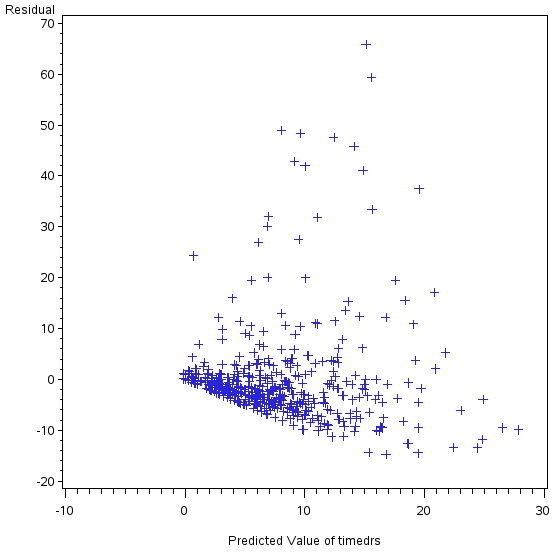
\includegraphics[]{regressx1-1-SAS-fig.png}
\end{document}
